\chapter{Outils formel}
\pagebreak

\section{Logique classique des propositions}
\subsection{Vocabulaire}

\begin{description}
\item[Déduction] $\models \alpha$ ssi$ \neg \alpha$ est contradictoire
\item[Absurde] $\phi$ est contradictoire ssi $\neg \phi$ est valide
\item[DAG]: Un graphe dirigé acyclique
\item[Taille(Arbre)] = $\{ tout les symboles + connecteurs \}$
\item[Var(Arbre)] = $\{ Toutes les feuilles \}$
\item[Sous formules(Arbres)] = $\{ T + \cup_{i=0}^k SousFormules(Arbre_i) \}$
\item[Interprétation]: $\omega$ de $PROP_{ps}$ est une application de PS dans ${0.1}$
\item[Sémantique]: $[| \phi |](\omega)$ d'une formule $\phi$ de $PROP_{ps}$ dans l'interprétation $\omega$ est une élément de ${0.1}$ définit inductive ment par:
\begin{description}
\item[$si \phi \in PS$] alors $[|\phi|](\omega) = \omega(\phi)$
\item[$si \phi = cX_1 ... X_n$] alors $[|\phi|](\omega) = C_F([|x_1|](\omega) ... [|x_n|](\omega))$
\end{description}
\item[$\omega $ satisfait $ \phi$] noté $\omega \models \phi $ssi$ [|\phi|](\omega) = 1$
\item[Lorsque $\omega \models \phi$] on dit que $\omega$ est un modèle de $\phi$
\item[on note $\eta(\phi)$] l'ensemble des modèles de $\phi$
\item[$\omega \in PROP_{ps}$ est valide] noté $\models \phi$, ssi toute interprétation$ \omega de PROP_{ps}$ satisfait$ \phi$
\item[$phi \equiv \psi$] sont logiquement équivalents ssi$ phi \models \psi$ et $psi \models \phi$
\end{description}

\subsection{Propriétés de l'opérateur Models}

\begin{description}
\item[$a \models b$] $=== M(a) \subseteq M(b)$
\item[Réflexivité]: $\phi \models \phi$
\item[Équivalence à gauche]: si $\phi \equiv \theta $et$ \phi \models \psi $alors$ \theta \models \psi$
\item[Affaiblissement à droite (transitivité)]: si$ \phi \models \psi $et$ \psi \models \theta $alors$ \phi \models \theta$
\item[Coupure]: si$ \phi \wedge \psi \models \theta $et$ \phi \models \psi $alors$ \phi \models \theta$ : $=== (A \cup B) \subseteq C ssi A \subseteq C \cap B \subseteq C$
\item[] 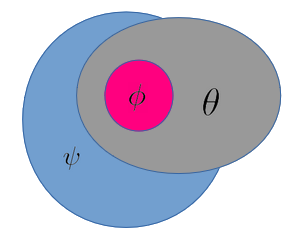
\includegraphics[scale=0.3]{img/of-coupure.png} 
\item[Ou]: $\phi \vee \psi \models \theta $ssi$ \phi \models \theta $et$ \psi \models \theta$
\item[] 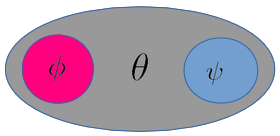
\includegraphics[scale=0.3]{img/of-ou.png}
\item[Monotonie]: si $\phi \models \theta $alors$ \phi \wedge \psi \models \theta$
\item[] 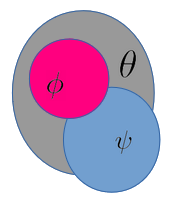
\includegraphics[scale=0.3]{img/of-monotomie.png}
\end{description}

\subsection{Ensemble de connecteurs fonctionnellement complet}
\begin{description}
\item[On dit qu'un ensemble est fonctionnellement complet] si avec que les connecteurs de cette ensemble on peut exprimer toutes les formules d'un monde.
\item[$\{\neg, \wedge\}$] est fonctionnellement complet pour la logique propositionnel classique
\item[] Il en va de même pour $\{\neg, \vee\}, \{vrai, \wedge, \bigoplus\}, \{\neg, \Rightarrow\} ou \{NAND\}$

\begin{description}
\item[Suppression des fils équivalent]: Soit un arbre D ayant comme sous arbre plus d'une fois le nœud $\alpha = (\top X \top)$, $\alpha$ peut être remplacé par $(\top)$ tout en concevant les modèles de D.
\item[fusion des nœuds]: Soit un arbre D ayant comme sous arbre les nœuds $(a B c)$ et $(a` B` c`)$ et $a = a`, b = b`, c = c`$ alors on peut faire relier les deux branches menant vers ces nœuds vers le même sous arbre.
\end{description}
\end{description}

\subsection{Preuve par induction structurelle sur un ensemble de connecteurs non fonctionnellement complet}

Soit $ \forall P \in \{ \wedge, \vee \}_{ps}$, vérifier P:
\begin{description}
\item[Cas de base $\varphi \in PS$]: $1^\rightarrow (\varphi) = 1$ donc $1^\rightarrow$ constitue un modèle de $\varphi$
\item[Étape inductive]: 
\begin{description}
\item[$\varphi$ s'écrit]: $[\alpha \wedge \beta]$ ou $[\alpha \vee \beta]$
\item[] Avec $\alpha, \beta \in \{ \wedge, \vee \}_{ps}$
\item[] Par hypothèse d'induction, $\alpha et \beta$ vérifient P.
\item[] Il ne reste plus qu'a montrer que $\varphi$ vérifie P.
\item[] $[| \alpha \vee \beta |)(1^\rightarrow)$ = $\vee \models ([|\alpha |)(1^\rightarrow), [|\beta |)(1^\rightarrow))$ = $\vee \models (1,1)$ = $1$
\item[] $[| \alpha \wedge \beta |)(1^\rightarrow)$ = $\wedge \models ([|\alpha |)(1^\rightarrow), [|\beta |)(1^\rightarrow))$ = $\wedge \models (1,1)$ = $1$
\item[] donc $x \wedge \neg x$ ne vérifie pas  $P: [| x \wedge \neg x|)(1^\rightarrow) = 0$
\end{description}
\end{description}

\subsection{Décomposition de Shannon}
\begin{description}
\item[On note $\phi [x \leftarrow 0 ) $ ] la formule obtenue en substituant dans $\phi$ la constante faux à toutes les occurrences du symbole propositionnel x.
\item[On note $\phi [x \leftarrow 1 ) $ ] la formule obtenue en substituant dans $\phi$ la constante vrai à toutes les occurrences du symbole propositionnel x.
\end{description}

La décomposition de Shannon de $\phi$ suivant x est la formule:
\begin{description}
\item[] $(\neg x \wedge \phi [x \leftarrow 0]) \vee (x \wedge \phi [x \leftarrow 1])$
\end{description}

\pagebreak
\subsection{Arbre de Shannon, ROBDD}
Étant donnée un ordre strict total $x_1 < x_2 < x_3$ sur $Var(\phi ) = \{x_1, ..... X_n\}$\\
Et une formule $\phi = (\neg x_1 \wedge x_2) \vee ( \neg x2 \wedge x_3)$\\\
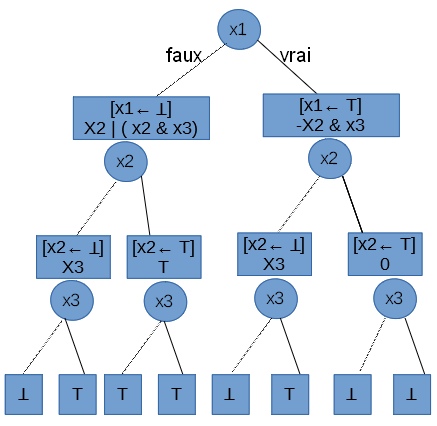
\includegraphics[scale=0.4]{img/of-arbre-shannon_1.png} \\
L'ensemble des modèles de $\phi$ sont toutes les interprétation où la feuille vaut la valeur $T$.

\subsubsection{Remplacement ou vérifonctionnalité}
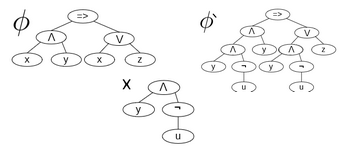
\includegraphics[scale=0.8]{img/of-remplacement.png} \\

$\phi \equiv \phi^{`}$ quelque soit la valeur de x (vrai ou faux).

\subsubsection{Substitution}
Soit un arbre $D$ ayant comme nœud un sous arbre du type infixe $\alpha = (x \Rightarrow y)$ et un sous arbre de substitution $\beta = (\neg x \Rightarrow \neg y)$\\
$(D^{`} = D_{\alpha \leftarrow \beta} \equiv D$)\\

\subsection{Notion de impliquant premier }

ggg

\subsection{Système de Hilbertein}

gg

\subsection{Forte complétude}

g

\pagebreak
